\documentclass[journal]{IEEEtran}
\usepackage{amsmath,amssymb,bm,mathtools}
\usepackage{booktabs,array,multirow}
\usepackage{graphicx}
\usepackage{cite}
\usepackage{url}
\usepackage[hidelinks]{hyperref}
\usepackage{balance}
\usepackage{tikz}
\usetikzlibrary{arrows.meta,positioning,fit,shapes.geometric}
\usepackage{algorithm}
\usepackage{algorithmic}
\usepackage{xcolor}
\newcommand{\EESS}{\mathrm{EESS}}
\newcommand{\PF}{\mathrm{PF}}
\newcommand{\R}{\mathbb{R}}
\newcommand{\I}{\mathcal{I}}
\newcommand{\U}{\mathcal{U}}
\newcommand{\B}{\mathcal{B}}
\newcommand{\M}{\mathcal{M}}
\newcommand{\tr}{\operatorname{tr}}
\newcommand{\diag}{\operatorname{diag}}
\newcommand{\argmin}{\operatorname*{arg\,min}}
\newcommand{\norm}[1]{\left\lVert #1\right\rVert}
\title{Predictive Bounded-Local Control for FR3 Spectrum Sharing: Safety, Utility, and Feasibility-Conditioned User Protection}
\author{Ali Fazeli and Raviraj S. Adve%
\thanks{The authors are with the Edward S. Rogers Sr. Department of Electrical and Computer Engineering, University of Toronto, Toronto, ON, Canada.}}
\begin{document}
\maketitle

\begin{abstract}
We study downlink resource management for an FR3 cellular network sharing spectrum with a protected Earth-exploration satellite service (EESS) earth station. The control problem combines delayed actuation, a 3-dB-per-update slew limit, simultaneous long- and short-horizon incumbent criteria, moving-average proportional fairness, and a practical 64-RF-chain/128-port array. We develop a predictive hierarchy that preserves fixed regularized-zero-forcing beam directions and uses only bounded local actions: incumbent-priced sector modes, sparse sector backoff, exact fixed-beam stream-power redistribution, and floor-first protected-subband scheduling. At fixed beams, both user-floor and EESS constraints become linear in stream powers; when simultaneous fixed-beam service is infeasible, a finite scheduling master problem convexifies the average-rate region and either returns a feasible slot mixture or an explicit unresolved certificate. In a frozen fresh holdout with 30 channel seeds, five pass blocks, and nine methods, the candidate improves final moving-PF utility over safe static control by $0.2505$ with a seed-cluster bootstrap 95\% interval $[0.2013,0.3102]$, and over the reviewed predictive controller by $0.0563$ with interval $[0.0205,0.0967]$. All 150 candidate pass cells have zero long- and short-horizon EESS violations, satisfy strict post-mode power constraints, and avoid network-wide shutdown. The unchanged user floor is met without violation in 17 of 30 seeds; over the full holdout, the hierarchy reduces floor-violation user-seconds by 81.47\% relative to predictive control and 84.76\% relative to safe static control. We therefore make a feasibility-conditioned floor claim and report the fixed-association serviceability limitation rather than weakening the floor.
\end{abstract}

\begin{IEEEkeywords}
FR3, spectrum sharing, EESS, predictive control, proportional fairness, massive MIMO, fixed RZF, distributed resource management, robust optimization.
\end{IEEEkeywords}

\section{Introduction}
Upper-mid-band spectrum can combine materially larger bandwidth than conventional sub-7-GHz systems with less severe propagation loss than millimeter-wave bands. That opportunity is accompanied by a difficult coexistence problem: FR3 allocations contain fixed links, satellite earth stations, scientific services, and other incumbents whose protection is defined at a third-party receiver rather than at a cooperating cellular terminal. A cellular controller must therefore manage utility and fairness while respecting interference constraints that are evaluated outside the cellular network.

Most beamforming formulations impose a static interference-temperature constraint on a single optimization instance. That abstraction is incomplete when the incumbent coupling changes along a satellite pass, control commands are delayed, and attenuation is slew limited. A reactive action that is safe at the current update can become unsafe before the next command takes effect. Static worst-case backoff avoids this failure but can sacrifice substantial user utility and fairness. These observations motivate a predictive safety layer that operates on practical radio-resource-management actions instead of repeatedly solving a centralized beam-space problem.

A second issue is exposed only after incumbent safety is made hard. Sector-wide attenuation can preserve EESS limits while leaving some active users below a service floor. A common sector scalar changes desired and same-sector interfering streams together and cannot in general repair a stream imbalance. Moreover, the simultaneous floor vector can be infeasible under fixed association even when each user is individually serviceable. Treating this as a small numerical error, weakening the floor after observing the data, or hiding it under sum-rate improvement would produce an indefensible paper.

This work develops and evaluates a bounded-local hierarchy for this coupled problem. The main contributions are:
\begin{enumerate}
\item A delayed and slew-limited predictive constrained-PF controller that uses future incumbent coupling, local fixed-RZF processing, incumbent-priced sector actions, and sparse emergency backoff under simultaneous long- and short-horizon EESS constraints.
\item An exact floor-feasibility repair at fixed beam directions. User SINR targets, EESS constraints, and sector power limits are linear in the stream-power scales, which permits a floor-first linear program with minimum action deviation as a secondary objective.
\item A protected-subband scheduling fallback that time-shares a finite mode library over physical 0.5-ms slots. The schedule preserves the frozen predictive mode trajectory and fixed RZF directions, uses bounded guard sectors, and returns a certificate when the declared action class remains infeasible.
\item A pre-specified, Git-frozen fresh 30-seed holdout with common random numbers, five fixed pass blocks, nine methods, and 10,000-replication seed-cluster bootstrap inference. The evaluation reports utility, both incumbent criteria, floor burden, action scope, power, runtime, payload lower bounds, and explicit claim boundaries.
\end{enumerate}

The holdout supports strong utility and incumbent-safety conclusions but not a universal user-floor guarantee. This distinction is central: the proposed controller enforces the unchanged floor when its declared bounded action set is feasible and quantifies unresolved serviceability otherwise.

\section{Related Work and Positioning}
Dynamic spectrum access and cognitive underlay control traditionally constrain the interference delivered to a primary receiver while maximizing secondary throughput~\cite{zhao2007dsa,ghasemi2007limits,zhang2008multiantenna}. These formulations established the value of interference-temperature constraints, multi-antenna spatial selectivity, and opportunistic reuse. They generally treat one optimization instant or a stationary fading law, whereas the present problem includes deterministic pass-dependent coupling, delayed commands, a slew limit, simultaneous long- and short-horizon criteria, and an explicit moving user-service floor.

Coordinated MIMO optimization provides a second reference point. Weighted-MMSE and related alternating methods can optimize network utility over beamformers under centralized or message-passing architectures~\cite{christensen2008weighted,shi2011wmmse,wagner2012large}. Re-solving the full beam space at every control update is intentionally outside the present architecture. Each sector constructs local RZF directions after a frozen hybrid mapping; higher layers operate on sector modes, sparse backoff, fixed-beam stream powers, and a finite scheduling library. This restriction lowers dimensionality and makes the modified sector set auditable, at the cost of a fixed-association serviceability boundary.

Safety filters, model-predictive control, and control barrier functions formalize hard-constraint enforcement under dynamics~\cite{rawlings2017mpc,ames2017cbf,ames2019theory,agrawal2017dcbf,jankovic2018robust,xiao2022hocbf}. The present contribution is not a new generic barrier-function theorem. It is a finite-pass reachability construction for third-party incumbent harm, coupled to wireless PF control and a hierarchy that either repairs user floors inside the declared radio action class or returns an unresolved certificate. The implemented safety statement is conditional on the frozen coupling envelope and physical model; it is not an infinite-horizon probabilistic or hardware-calibrated guarantee.

FR3 studies emphasize the propagation, array, and coexistence questions that arise above conventional sub-7-GHz bands~\cite{kang2024upper,chamberlain2024sharing}. The cellular realization follows 3GPP TR~38.901 using Sionna~\cite{3gpp38901,hoydis2022sionna}; incumbent coupling and engineering criteria use the explicitly frozen ITU-R roles in Section~\ref{sec:model}~\cite{iturp452,itursa1027,itursa509,iturf758}. Table~\ref{tab:positioning} summarizes the resulting position: the work is neither static exclusion nor centralized beam optimization, but a predictive bounded-local hierarchy with explicit failure semantics.

\begin{table*}[t]
\caption{Positioning relative to common coexistence-control abstractions.}
\label{tab:positioning}
\centering
\footnotesize
\setlength{\tabcolsep}{4.0pt}
\renewcommand{\arraystretch}{1.05}
\begin{tabular}{@{}p{0.19\textwidth}p{0.23\textwidth}p{0.24\textwidth}p{0.25\textwidth}@{}}
\toprule
Class & Strength & Missing element for this problem & Role in this work\\
\midrule
Static exclusion/backoff & Simple, auditable incumbent protection & Ignores drift, delay, and unnecessary persistent conservatism & Safe-static and uniform baselines\\
Interference-constrained beam optimization & Efficient spatial reuse when centralized CSI and beam control are available & Re-solves beam space and obscures bounded action scope & Non-deployable reference point; fixed RZF retained\\
Generic safety filter / MPC & Handles state evolution and hard constraints & Does not specify third-party propagation, user floors, or fixed-association serviceability & Predictive reachability envelope and conditional safety result\\
Proposed hierarchy & Prediction, exact fixed-beam repair, time sharing, and explicit failure semantics & Does not solve association or certify standardized messaging latency & Evaluated candidate and stated claim boundary\\
\bottomrule
\end{tabular}
\end{table*}


\section{System and Protection Model}
\label{sec:model}
\subsection{Network and practical array}
The evaluated platform has 19 sites, three sectors per site, 57 sectors, and 228 users. Each sector is represented by 128 dual-polarized physical ports and a generic practical mapping with 64 RF chains, 32 disjoint dual-polarized subarrays, and 6-bit analog phase control. Local digital RZF is computed after the analog network. The observed minimum remaining digital dimension in the frozen architecture is 58, and no local-rank failure occurs in the evaluated topology.

Let $b\in\B$ denote a sector, $k$ a local RZF stream, $f$ a protected frequency group, and $t$ the 5-s control interval. The protected-subband transmit covariance is
\begin{equation}
 \bm Q_{b,t}=\rho_{b,t}\sum_{k}x_{b,k,t}
 \bm w_{b,k,t}\bm w_{b,k,t}^{H},
 \label{eq:covariance}
\end{equation}
where $\bm w_{b,k,t}$ is a frozen RZF direction, $\rho_{b,t}\in[0,1]$ is the reviewed sector fallback scale, and $x_{b,k,t}\in[0,1]$ is an optional stream-power multiplier. The primary hierarchy never changes $\bm w_{b,k,t}$ and never uses power beyond the strict post-mode sector envelope.


\subsection{Hybrid-array action mapping}
The analog network is frozen for the campaign. Each dual-polarized subarray feeds two RF chains and the 6-bit phase settings are fixed by the architecture construction. Protected-mode commands act after this network. The digital RZF columns therefore capture the residual spatial degrees of freedom available to the controller, while the power and scheduling variables in \eqref{eq:covariance} remain implementable as baseband stream weights and protected-subband scheduling decisions.

This separation is important for claim discipline. A 65-dB declared null-depth cap is applied to the mode model, but the controller never assumes that an arbitrary 128-port covariance can be realized. Conversely, the fixed-beam repair does not consume array degrees of freedom that the practical mapping does not have. Per-mode sector power is reconstructed from the actual post-mode precoder, and each candidate schedule mode is rejected if its stream coefficients would exceed that envelope.

The local-RZF architecture also creates the same-sector fairness issue that motivates stream repair. If sector $b$ applies only a common scale $\rho_b$, then the desired stream and all same-sector interferers of a user are changed proportionally. A weak stream may therefore remain below its floor even when the sector has enough total protected-subband power. The vector $\{x_{b,k}\}_k$ adds selectivity without changing beam directions.

\begin{table*}[t]
\caption{Frozen propagation, radio, traffic, control, and statistical settings.}
\label{tab:parameters-expanded}
\centering
\footnotesize
\setlength{\tabcolsep}{4.3pt}
\renewcommand{\arraystretch}{1.05}
\begin{tabular}{@{}p{0.20\textwidth}p{0.27\textwidth}p{0.20\textwidth}p{0.27\textwidth}@{}}
\toprule
Item & Setting & Item & Setting\\
\midrule
Topology & 19 sites, 57 sectors, 4 users/sector & Channel scenario & 3GPP TR~38.901 UMa\\
Carrier / total BW & 8.15 GHz / 100 MHz & Protected group & Center 10 MHz of nine groups\\
User radius / indoor prob. & 50--200 m / 0.8 & BS power / UE NF & 46 dBm per 100 MHz / 7 dB\\
Array & $8\times8$ dual-pol., 128 ports & Hybrid mapping & 64 RF chains, 32 dual-pol. subarrays, 6-bit phases\\
Local precoding & Fixed-direction digital RZF & Engineering envelope & 65-dB null-depth cap, 3-dB coupling uplift\\
Long criterion & P.452 $p=20\%$, $-150$ dBW/10 MHz & Short criterion & P.452 $p=0.005\%$, $-133$ dBW/10 MHz\\
Update / delay / slew & 5 s / one update / 3 dB/update & Moving-PF memory & 100-s exponential average\\
Load sequence & $4,2,4,1,3,2$ streams/sector & Phase lengths & $20,20,20,20,20,18$ intervals + extension\\
Floor / eligibility & $\max\{0.1,0.9R^{\rm nom,current}\}$ / full-load $\ge0.1$ & Holdout / inference & 30 fresh seeds, five fixed passes, 10,000 seed-cluster resamples\\
\bottomrule
\end{tabular}
\end{table*}


\begin{figure*}[t]
\centering
\resizebox{0.98\textwidth}{!}{%
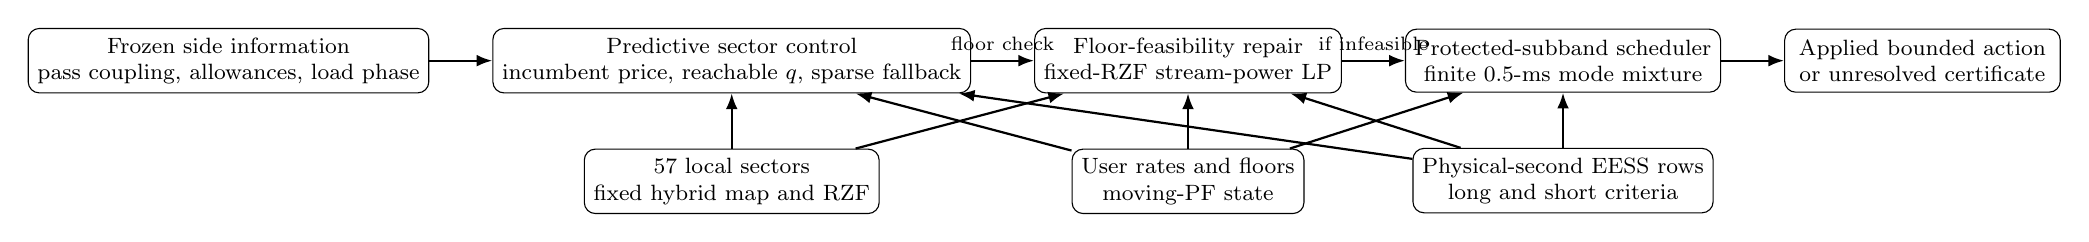
\begin{tikzpicture}[
  node distance=5mm and 8mm,
  box/.style={draw,rounded corners,align=center,minimum height=8mm,minimum width=27mm,font=\footnotesize},
  wide/.style={box,minimum width=35mm},
  arr/.style={-{Latex[length=2mm]},thick},
  note/.style={font=\scriptsize,align=center}
]
\node[wide] (side) {Frozen side information\\pass coupling, allowances, load phase};
\node[wide,right=of side] (pred) {Predictive sector control\\incumbent price, reachable $q$, sparse fallback};
\node[wide,right=of pred] (lp) {Floor-feasibility repair\\fixed-RZF stream-power LP};
\node[wide,right=of lp] (sched) {Protected-subband scheduler\\finite 0.5-ms mode mixture};
\node[wide,right=of sched] (out) {Applied bounded action\\or unresolved certificate};
\draw[arr] (side) -- (pred);
\draw[arr] (pred) -- node[above,note]{floor check} (lp);
\draw[arr] (lp) -- node[above,note]{if infeasible} (sched);
\draw[arr] (sched) -- (out);
\node[box,below=7mm of pred] (local) {57 local sectors\\fixed hybrid map and RZF};
\node[box,below=7mm of lp] (users) {User rates and floors\\moving-PF state};
\node[box,below=7mm of sched] (eess) {Physical-second EESS rows\\long and short criteria};
\draw[arr] (local) -- (pred);
\draw[arr] (local) -- (lp);
\draw[arr] (users) -- (pred);
\draw[arr] (users) -- (lp);
\draw[arr] (users) -- (sched);
\draw[arr] (eess) -- (pred);
\draw[arr] (eess) -- (lp);
\draw[arr] (eess) -- (sched);
\end{tikzpicture}}
\caption{Controller hierarchy. Beam directions and the hybrid mapping remain local and frozen. Low-dimensional sector actions are screened against future incumbent coupling; exact fixed-beam repair and finite protected-subband scheduling are invoked only when the preceding layer cannot satisfy the unchanged user floors.}
\label{fig:architecture}
\end{figure*}

\subsection{EESS criteria}
The EESS case is an 8.15-GHz engineering scenario with the aggregate interference power referenced to 10 MHz. The long-horizon criterion uses P.452 $p=20\%$ and $-150$ dBW/10 MHz; the short-horizon criterion uses P.452 $p=0.005\%$ and $-133$ dBW/10 MHz. The primary earth-station pattern is the SA.509 multiple-entry pattern, with the single-entry pattern retained as a conservative sensitivity in the underlying platform. These are deterministic engineering tests, not a calibration or regulatory-compliance certificate~\cite{iturp452,itursa1027,itursa509}.

For physical second $s$ within interval $t$, let $\kappa^{c}_{s,b}$ be the time-varying coupling coefficient for criterion $c\in\{L,S\}$, $\ell_{b,k,t}$ the post-mode leakage of stream $(b,k)$, $A^{c}_{s}$ the allowed aggregate power, and $\chi$ the declared 3-dB coupling uplift. The normalized ratio is
\begin{equation}
 e^{c}_{s,t}(\bm x_t)=
 \frac{\chi\sum_{b,k}\kappa^{c}_{s,b}\ell_{b,k,t}x_{b,k,t}}
 {A^{c}_{s}}.
 \label{eq:eess}
\end{equation}
The hard safety condition is $e^{c}_{s,t}\le 1$ for every evaluated second and for both criteria. The predictive controller uses the future coupling envelope to anticipate the one-update delay and the 3-dB/update attenuation slew.

\subsection{Moving proportional fairness and user floor}
Let $R_{u,t}$ be the total-band rate of user $u$ and $\bar R_{u,t}$ its exponential moving average with a 100-s time constant. Inactive backlogged users receive a zero-rate update. The controller's utility is the moving-PF objective
\begin{equation}
 J_t=\sum_{u\in\U}\log\!\left(\bar R_{u,t}+\epsilon\right),
 \label{eq:pf}
\end{equation}
not instantaneous sum rate. A user is eligible if its full-load nominal total-band rate is at least 0.1 bit/s/Hz. For every active eligible user, the unchanged floor is
\begin{equation}
 F_{u,t}=\max\!\left\{0.1,\;0.9R^{\mathrm{nom,current}}_{u,t}\right\}.
 \label{eq:floor}
\end{equation}
The current-load nominal reference follows the same load phase and channel realization but removes incumbent-protection action. Equation~\eqref{eq:floor} is not relaxed after observing a difficult seed.

\section{Predictive Bounded-Local Control}
\subsection{Reviewed predictive controller}
At every update, each sector evaluates a local table of admissible protected modes and sector scales. The local PF cost uses the predicted moving-rate update, while an incumbent price penalizes the sector's predicted contribution to the future EESS envelope. The coordinator updates the price and selects a reachable action under the one-update command delay and 3-dB slew. A sparse sector-selective fallback is invoked if the reviewed action cannot satisfy both EESS criteria.

This architecture differs from centralized beam optimization in two ways. First, RZF directions remain local and frozen over the repair. Second, coordination is confined to low-dimensional attenuation, sparse backoff, and later a bounded set of scheduling guards. The unsafe delayed-myopic and virtual-queue methods are retained only as negative controls because they do not impose the physical-second EESS constraints.

\subsection{Exact fixed-beam stream-power repair}
At fixed directions and fixed predictive modes, the received power from stream $j$ at user $u$ can be written as $g_{u,j}x_j$. Let $d(u)$ denote the desired stream. If the protected-subband rate needed to reach $F_{u,t}$ is $r^{\rm req}_{u,t}$, define $\gamma_{u,t}=2^{r^{\rm req}_{u,t}}-1$. The floor is equivalent to
\begin{equation}
 g_{u,d(u)}x_{d(u)}
 \ge \gamma_{u,t}\!\left(
 \sum_{j\ne d(u)}g_{u,j}x_j+N_0\right),
 \label{eq:linear-floor}
\end{equation}
which is linear in $\bm x$. Equation~\eqref{eq:eess} is also linear, and the strict post-mode power envelope is
\begin{equation}
 \sum_k P_{b,k,t}x_{b,k,t}\le \rho_{b,t}\sum_k P_{b,k,t}.
 \label{eq:power-envelope}
\end{equation}
The repair LP therefore imposes all active eligible floors, every physical-second EESS row, \eqref{eq:power-envelope}, $0\le x_j\le1$, and strict bounded-local scope. Feasibility is the first objective; a weighted $\ell_1$ distance from the reviewed action is minimized second. Sum rate is not used to trade away a floor or an EESS constraint.

\textbf{Proposition 1.} For fixed RZF directions, fixed protected modes, and a fixed active-user set, the joint floor, EESS, and sector-power feasibility problem is a linear program in the stream-power multipliers.

\emph{Proof sketch:} The SINR transformation in \eqref{eq:linear-floor} is affine after cross multiplication because all gains and noise terms are fixed. Equations~\eqref{eq:eess} and \eqref{eq:power-envelope} are linear by construction, and the box/locality constraints are polyhedral.

\subsection{Protected-subband scheduling}
Simultaneous fixed-beam service can be infeasible even when every user is individually serviceable. The scheduling fallback constructs modes $m\in\M_t$. A mode preserves the predictive $q$ state and fixed RZF directions but may serve selected streams alone in a critical sector and mute a bounded set of external guard sectors. Candidate v4.5 completes the singleton basis for active companion streams in each critical sector and permits a guard union selected from the ranked external pool.

Let $R_{u,m}$ and $e^{c}_{s,m}$ be the rate and normalized EESS ratio of mode $m$. The continuous master problem is
\begin{subequations}
\begin{align}
 \min_{\bm\tau}\quad &\sum_{m\in\M_t}c_m\tau_m\\
 \text{s.t.}\quad
 &\sum_m\tau_m R_{u,m}\ge F_{u,t}+\delta_R,\quad \forall u,\\
 &\sum_m\tau_m e^{c}_{s,m}\le 1-\delta_E,\quad \forall s,c,\\
 &\sum_m\tau_m=1,\qquad \tau_m\ge0,
\end{align}
\label{eq:schedule-lp}
\end{subequations}
where $\delta_R$ and $\delta_E$ are solver-side interior reserves, not relaxed scientific tolerances. A 0.5-ms physical schedule uses $N=2000$ slots per second and integer counts $n_m$ satisfying the corresponding MILP with $\sum_m n_m=N$.

\textbf{Proposition 2.} Any accepted integer schedule satisfies the unchanged average user floors, both physical-second EESS constraints, and per-mode post-mode power limits under the declared mode library.

\emph{Proof sketch:} The scheduled rate and leakage are convex combinations of pre-audited mode quantities. The integer master enforces the same rows as \eqref{eq:schedule-lp} after multiplication by $N$, and every generated mode is independently checked against the post-mode sector-power envelope.

\subsection{Hierarchy and infeasibility certificate}
The complete action hierarchy is:
\begin{enumerate}
\item reviewed predictive mode/sector fallback;
\item sparse frozen-grid sector repair;
\item fixed-RZF stream-power LP with bounded external/EESS contributors;
\item protected-subband scheduling with bounded guards;
\item an unresolved certificate if the declared fixed-association action set has no accepted witness.
\end{enumerate}
The certificate is important. It prevents a numerical optimizer from silently reducing the floor and distinguishes controller failure from fixed-association serviceability. User reassignment, multi-connectivity, and serviceability-aware admission are valid future extensions, but they are not introduced post hoc in the present holdout.

\begin{algorithm}[t]
\caption{Bounded-local predictive control and floor repair}
\label{alg:hierarchy}
\begin{algorithmic}[1]
\STATE Build delayed reachability envelopes for both EESS criteria.
\STATE Select reachable sector modes using local moving-PF costs and the incumbent price.
\IF{either physical-second EESS screen fails}
  \STATE invoke sparse sector fallback; reject if safety remains infeasible.
\ENDIF
\STATE Evaluate all active eligible user floors under the reviewed action.
\IF{all floors pass}
  \STATE accept the reviewed action.
\ELSE
  \STATE test sparse sector-grid repair, then the fixed-RZF stream-power LP.
  \IF{a fixed-beam witness passes exact recomputation}
    \STATE accept the minimum-deviation witness.
  \ELSE
    \STATE solve the protected-subband scheduling master and integer slot allocation.
    \IF{the exact schedule passes floor, EESS, power, and scope gates}
      \STATE accept the schedule.
    \ELSE
      \STATE retain safety and return an unresolved serviceability certificate.
    \ENDIF
  \ENDIF
\ENDIF
\STATE Apply the delayed command and update every user's moving rate, including zeros for inactive backlogged users.
\end{algorithmic}
\end{algorithm}


\subsection{Lexicographic objective and local action scope}
The hierarchy is lexicographic rather than a weighted sum of incompatible goals. Its ordering is:
\begin{equation}
\begin{aligned}
&\text{(i) satisfy both EESS criteria,}\\
&\text{(ii) satisfy every active eligible floor when feasible,}\\
&\text{(iii) minimize changed-action count and magnitude,}\\
&\text{(iv) retain moving-PF utility.}
\end{aligned}
\label{eq:lexicographic}
\end{equation}
Consequently, a large utility coefficient cannot purchase an incumbent violation or intentionally leave a feasible floor unsatisfied. The implementation realizes this ordering through feasibility subproblems and only then an action-deviation objective.

For an initially violating user, external sectors are ranked by received interference and sectors contributing to EESS are ranked by leakage. The strict local repair permits the serving sector, at most two dominant external interferers per affected user, and at most two dominant EESS contributors. The scheduling extensions use a larger but still explicit guard pool and cap the union of mute-only guards. Every accepted action records the mutable-sector set. This creates an auditable action-scope notion of locality. It does not, by itself, prove that the messages needed to rank those sectors can be exchanged within a specified standardized interface.

\subsection{Predictive information pattern}
At update $t$, the applied action is the command issued one update earlier. The controller has the frozen future coupling envelope over the protected pass, but no future cellular small-scale channel beyond the common simulation realization. For a candidate local action $a_{b,t}$, a sector constructs a cost
\begin{equation}
 C_{b,t}(a_{b,t})=
 -\sum_{u\in\U_b}\log\!\left(\bar R_{u,t+1}(a_{b,t})+\epsilon\right)
 +\lambda_t \widehat I_{b,t+1}(a_{b,t}),
 \label{eq:local-cost}
\end{equation}
where $\lambda_t$ is the incumbent price and $\widehat I_{b,t+1}$ uses the delayed reachable action and the preloaded coupling. The coordinator does not optimize beam matrices; it combines scalar/mode contributions and updates the price until the hard reachability screen is met or the fallback is invoked.

A safe-static controller uses a fixed conservative action across the pass. The delayed reactive controller uses the same local cost and fallback but does not anticipate the future coupling. This construction gives the predictive and reactive methods matched action spaces and fallback logic, isolating the value of prediction.


\subsection{Predictive safety property}
For criterion $c$, let $\overline{\bm c}^{c}_{i}\in\R_{+}^{57\times2}$ collect the upper-bounded sector--mode contributions in interval $i$, before the selected attenuation. Let $d$ be the command delay in update intervals, $\Delta_q$ the maximum attenuation increase per update, and $\alpha=10^{-\Delta_q/10}$. The implementation constructs an elementwise backward application envelope
\begin{equation}
 \bm h^{c}_{i}=\max\!\left\{\overline{\bm c}^{c}_{i},\;\alpha\bm h^{c}_{i+1}\right\},
 \qquad \bm h^{c}_{T}=\overline{\bm c}^{c}_{T},
 \label{eq:application-envelope}
\end{equation}
and the delayed command envelope $\bm g^{c}_{t}=\bm h^{c}_{\min\{t+d,T\}}$. The controller chooses one reachable command $\bm q_t\in\mathcal A(\bm q_{t-1})$ satisfying
\begin{equation}
 \frac{\left\langle\bm g^{c}_{t},10^{-\bm q_t/10}\right\rangle}{A^{c}_{t}}
 \le 1,\qquad \forall c,
 \label{eq:predictive-screen}
\end{equation}
where the exponential is elementwise. Equation~\eqref{eq:predictive-screen} screens the \emph{selected} reachable action against an envelope that already accounts for the delay and all future contributions reachable under the slew; it does not require every reachable action to be safe.

\textbf{Proposition 3.} Suppose $\overline{\bm c}^{c}_{i}$ upper bounds the realized contribution tensor under the declared model, the envelope obeys \eqref{eq:application-envelope}, and the selected commands obey the reachability and screen constraints. Then the applied action satisfies the normalized EESS bound over the certified finite pass for criterion $c$.

\emph{Proof sketch:} Nonnegative leakage makes the EESS ratio monotone in every contribution coefficient. The backward recurrence dominates the current upper contribution and the most adverse contribution remaining after one additional slew-limited attenuation step. Shifting the application envelope by the command delay yields the contribution against which the selected command is tested. Induction over the finite pass, including the preloaded action, then gives the physical-second upper bound. The certificate is conditional on the declared coupling envelope and finite pass; it is neither an infinite-horizon chance guarantee nor a hardware calibration.

The reviewed simulation evaluates both criteria at every physical second, not only at 5-s command boundaries. This is why an unshielded delayed controller can accumulate violation seconds even when its interval-end command appears reasonable.

\subsection{Failure semantics}
Three outcomes are distinguished:
\begin{enumerate}
\item \emph{safe and floor feasible}: all hard rows pass;
\item \emph{safe but floor unresolved}: both EESS criteria and power/locality gates pass, but at least one active eligible floor has no accepted witness in the declared action set;
\item \emph{unsafe}: at least one physical-second EESS row fails.
\end{enumerate}
Only the first two are valid candidate outcomes. The second is retained in the statistics and contributes its measured shortfall; it is never recoded as a successful floor event. An unsafe outcome would fail the candidate safety gate.

\section{Experimental Methodology}
\subsection{Frozen topology, passes, and information sets}
The cellular topology is generated once per seed and reused across all five fixed pass blocks and all methods. The pass blocks are deterministic geometry/load blocks rather than independent draws from an orbital-pass population. The control update is 5 s, the command delay is one update, and attenuation changes by at most 3 dB per update. The development campaign uses seeds 44000--44029. Candidate v4.5 is frozen after that development and then evaluated, without adaptation, on fresh seeds 44030--44059.

Common random numbers are used within each seed. Every method sees the same cellular channel, pass geometry, load sequence, and declared coupling envelope. The candidate and safe methods are required to satisfy both EESS criteria; the unshielded methods serve as negative controls.

\subsection{Methods}
Nine methods are evaluated:
\begin{enumerate}
\item candidate v4.5 predictive hierarchy;
\item reviewed predictive constrained PF with sector-selective fallback;
\item safe static constrained PF with the same fallback;
\item delayed reactive-myopic constrained PF with the same fallback;
\item delayed unshielded myopic control;
\item an unshielded virtual queue;
\item uniform protected-tone backoff;
\item hard spatial null or exact mute;
\item an instantaneous noncausal common-sector-scale reference.
\end{enumerate}
The noncausal reference is diagnostic, not deployable. The unshielded controls establish that high utility without hard physical-second protection is not an acceptable solution.

\subsection{Baseline matching and interpretation}
The candidate, reviewed predictive method, and reactive shielded method use the same local PF cost tables, protected-mode grid, slew limit, delay model, and sector-selective fallback. The predictive--reactive contrast therefore isolates anticipation of future incumbent coupling; the candidate--predictive contrast isolates fixed-beam floor repair and scheduling. Safe static uses the same engineering constraints but holds a single conservative action over the pass.

Uniform backoff and hard null/mute represent simple protection policies. The noncausal common-scale reference sees the instantaneous future requirement but is restricted to one sector-common scale, so it tests whether future information alone is sufficient. The two unshielded controllers are negative controls: their utility is reported, but any EESS violation makes them unacceptable operating points. No baseline is allowed a larger power envelope, a different channel, or a different load realization.

\subsection{Endpoints and inference}
The primary endpoint is the final moving-average sum-log utility. The mandatory secondary endpoint is the duration-weighted mean moving-PF utility. The primary paired comparison is candidate minus safe static. For each seed, the five pass effects are averaged, and 30 seed clusters are bootstrapped 10,000 times. No seed is excluded or imputed based on outcome. We also report candidate-minus-predictive effects, pass-specific effects, leave-one-pass-out intervals, p05 rates, floor burden, safety violations, action incidence, and runtime.

The fresh-holdout decision and analysis contract were Git-frozen before execution. A positive primary confidence interval and complete EESS safety authorize paper writing. Universal floor success was not a condition for validity because the final claim is explicitly feasibility conditioned.


\subsection{Load phases and floor accounting}
The deterministic activity sequence alternates full and reduced loads and includes a variable terminal extension. Eligibility is computed once from the full-load nominal rate, whereas the relative branch of \eqref{eq:floor} uses the current-load nominal rate. This distinction prevents a low-load interval from redefining which users count, but it can make the absolute 0.1-bit/s/Hz branch active for a user whose current-load nominal rate is lower than 0.1. Such intervals are not removed from the analysis.

Floor burden is measured in two ways. A \emph{user-interval} counts one active eligible user below its floor during one 5-s action interval. A \emph{user-second} multiplies that event by the physical duration represented by the interval. The maximum normalized shortfall is
\begin{equation}
 \Delta_{\max}=\max_{u,t:F_{u,t}>0}
 \frac{[F_{u,t}-R_{u,t}]_+}{F_{u,t}}.
 \label{eq:shortfall}
\end{equation}
This retains both incidence and severity.

\subsection{Reproducibility and exclusion policy}
Every seed is analyzed regardless of whether the candidate, a comparator, or a validator exits with a scientific nonzero code. Infrastructure failures are recovered without changing the channel. Seed 44052, for example, required pass-parallel completion because a monolithic job hit its wall-time after the declared scheduling library grew to 7,776 modes. The five pass blocks are independent from the same initialized moving-rate state; splitting them changes execution only, not the scientific calculation. The completed seed shifted the 30-seed primary mean by only $1.60\times10^{-4}$.

The holdout contains no outcome-based exclusion, no replacement seed, and no algorithm adaptation. All file-level manifests, seed-result hashes, and source manifests are archived.

\section{Results}
\subsection{Fresh-holdout utility and safety}
\begin{table}[t]
\caption{Fresh 30-seed holdout: claim-critical results.}
\label{tab:holdout-key-v2}
\centering
\footnotesize
\setlength{\tabcolsep}{3.0pt}
\renewcommand{\arraystretch}{1.06}
\begin{tabular}{@{}lr@{}}
\toprule
Metric & Result\\
\midrule
Candidate $-$ safe-static final PF & $0.2505$\\
Seed-cluster bootstrap 95\% CI & $[0.2013,0.3102]$\\
Candidate $-$ predictive final PF & $0.0563$\\
Seed-cluster bootstrap 95\% CI & $[0.0205,0.0967]$\\
Long-/short-horizon EESS violations & $0/0$\\
Safety-passing seeds & $30/30$\\
Zero-floor seeds & $17/30$\\
Floor reduction vs. predictive & $81.47\%$\\
Floor reduction vs. safe static & $84.76\%$\\
Unresolved scheduling intervals & $1{,}328$\\
\bottomrule
\end{tabular}
\end{table}

\begin{table}[t]
\caption{Development and fresh-holdout paired effects. Development seeds were used for candidate construction; the holdout was frozen before execution.}
\label{tab:dev-holdout}
\centering
\footnotesize
\setlength{\tabcolsep}{3.1pt}
\renewcommand{\arraystretch}{1.08}
\begin{tabular}{@{}lcc@{}}
\toprule
Effect & Development & Fresh holdout\\
\midrule
Final PF: candidate $-$ safe static &
$0.2883$ & $0.2505$\\
95\% seed-cluster CI &
$[0.2402,0.3382]$ & $[0.2013,0.3102]$\\
Final PF: candidate $-$ predictive &
$0.0610$ & $0.0563$\\
95\% seed-cluster CI &
$[0.0244,0.1010]$ & $[0.0205,0.0967]$\\
Duration PF: candidate $-$ safe static &
-- & $0.2088$\\
95\% seed-cluster CI &
-- & $[0.1767,0.2415]$\\
\bottomrule
\end{tabular}
\end{table}


The final moving-PF advantage over safe static is $0.2505$ and its 95\% seed-cluster interval is $[0.2013,0.3102]$. The corresponding duration-weighted advantage is $0.2088$ with interval $[0.1767,0.2415]$. Relative to the reviewed predictive controller, the final and duration-weighted effects are $0.0563$ and $0.0360$, with both 95\% intervals above zero. The development-to-holdout reduction in effect size is moderate and expected after freezing; the independent holdout remains statistically decisive.

All 30 candidate seed results and all 150 candidate pass cells are present. Long- and short-horizon EESS violations are zero, strict local action-scope and post-mode power gates pass, no network-wide shutdown occurs, and no deployable action relies on the broader $q=0$ power headroom. These facts support incumbent safety within the declared simulated envelope, not physical calibration or regulatory compliance.

\begin{figure}[t]
\centering
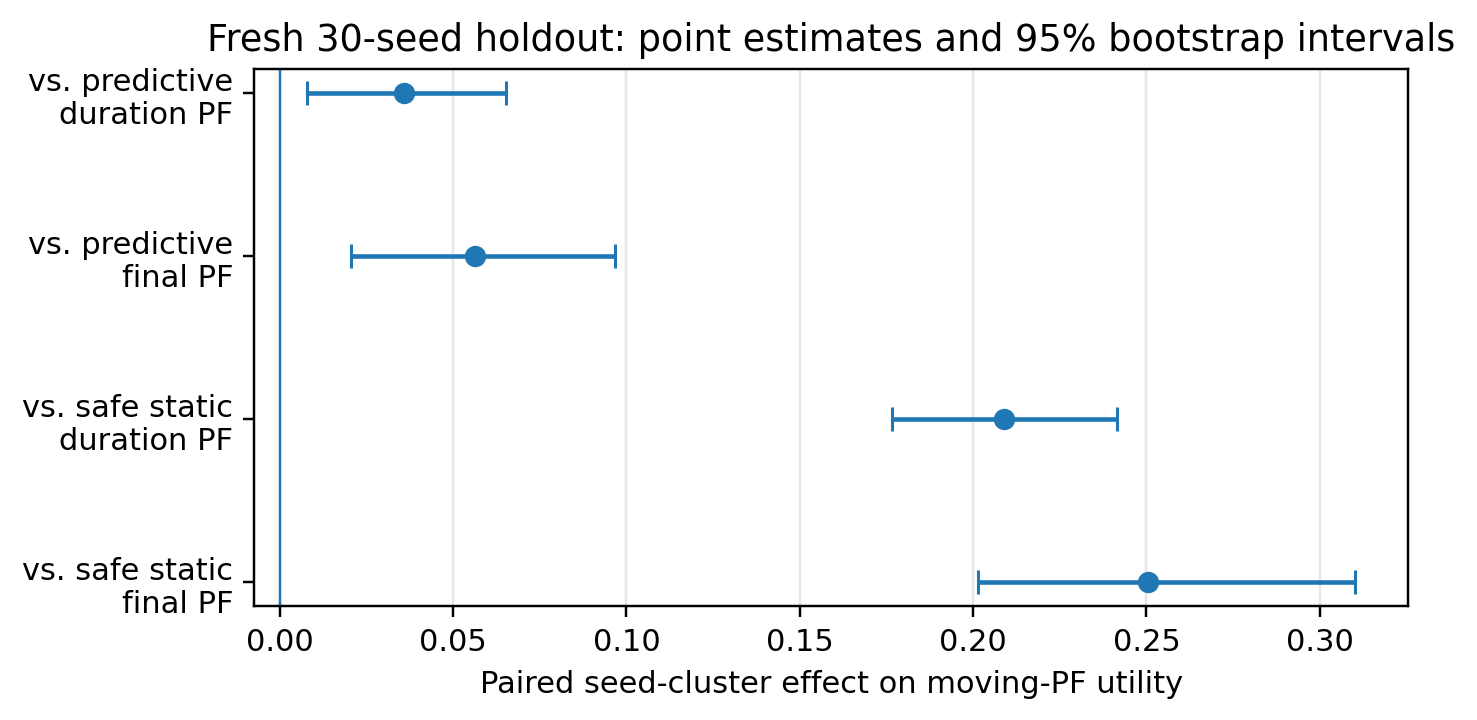
\includegraphics[width=\columnwidth]{figures/holdout_utility_effects.png}
\caption{Fresh-holdout paired effects. Error bars are 95\% seed-cluster bootstrap intervals over 30 fresh channel seeds.}
\label{fig:utility-effects}
\end{figure}

\begin{figure}[t]
\centering
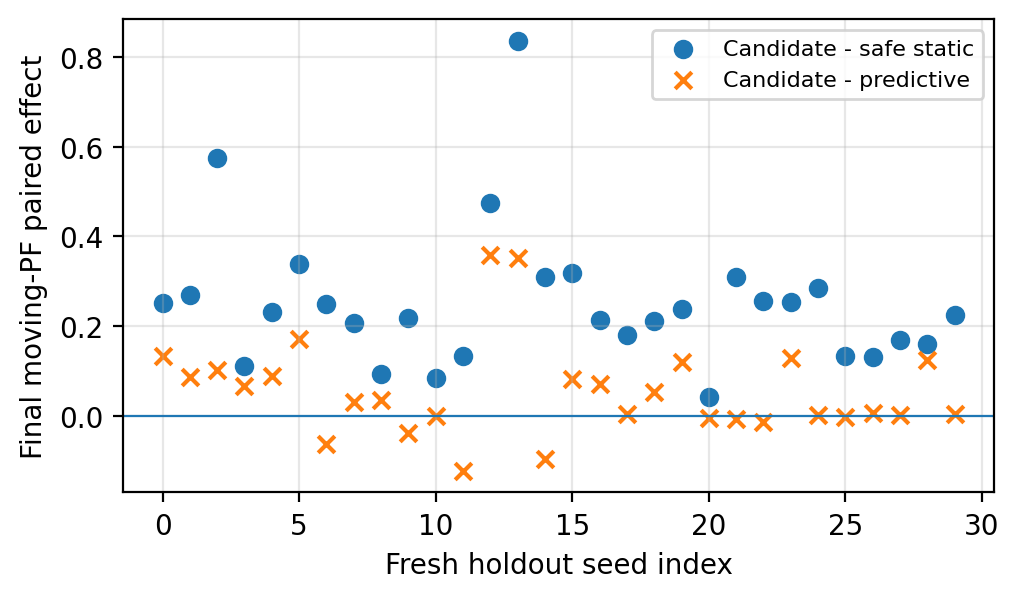
\includegraphics[width=\columnwidth]{figures/holdout_seed_effects.png}
\caption{Seed-level final moving-PF effects. Population-average intervals are positive, but pointwise dominance is neither required nor claimed.}
\label{fig:seed-effects}
\end{figure}

\subsection{Method comparison}
\begin{table*}[t]
\caption{Fresh-holdout comparison over 150 seed--pass cells. EESS entries are mean physical violation seconds per cell; floor burden is mean active-eligible user-seconds below the unchanged floor. Unshielded methods are negative controls, not acceptable operating points.}
\label{tab:method-comparison-full}
\centering
\footnotesize
\setlength{\tabcolsep}{4.6pt}
\renewcommand{\arraystretch}{1.06}
\begin{tabular}{@{}lrrrr@{}}
\toprule
Method & Final moving-PF & Long EESS & Short EESS & Floor burden\\
\midrule
Candidate v4.5 & 46.4043 & 0.0 & 0.00 & 111.0\\
Predictive & 46.3480 & 0.0 & 0.00 & 598.8\\
Safe static & 46.1538 & 0.0 & 0.00 & 728.1\\
Reactive + shield & 46.3286 & 0.0 & 0.00 & 604.3\\
Myopic, unshielded & 46.2851 & 145.1 & 0.06 & 604.8\\
Virtual queue, unshielded & 46.2026 & 152.3 & 0.00 & 625.3\\
Uniform backoff & 45.7934 & 0.0 & 0.00 & 606.7\\
Hard null/mute & 43.3730 & 0.0 & 0.00 & 2433.7\\
Noncausal common scale & 46.1341 & 0.0 & 0.00 & 797.3\\
\bottomrule
\end{tabular}
\end{table*}


Table~\ref{tab:method-comparison-full} shows that the candidate has the largest mean final moving-PF utility among the evaluated methods while preserving hard EESS safety. Safe static, uniform backoff, hard null/mute, and the noncausal common-scale reference are all EESS safe but have lower utility and substantially larger floor burden. The unshielded myopic and virtual-queue controls retain many long-horizon violation seconds, confirming that queue pressure alone does not replace a physical safety constraint.

The noncausal common-scale reference also has more floor burden than the predictive candidate. Future knowledge is therefore insufficient when the action class remains a single sector-common scale. The gain arises from action selectivity and floor-first feasibility, not simply from prediction.


\begin{table*}[t]
\caption{Fresh-holdout active-eligible rate summaries averaged over pass cells.}
\label{tab:rate-summary}
\centering
\footnotesize
\setlength{\tabcolsep}{5.0pt}
\renewcommand{\arraystretch}{1.08}
\begin{tabular}{@{}lrrrr@{}}
\toprule
Method & Protected p05 & Protected geometric mean & Total-band p05 & Total-band geometric mean\\
\midrule
Candidate v4.5 & 0.181 & 1.937 & 0.276 & 2.201\\
Predictive & 0.180 & 1.944 & 0.276 & 2.200\\
Safe static & 0.176 & 1.923 & 0.275 & 2.198\\
Uniform & 0.182 & 1.926 & 0.276 & 2.197\\
Hard null/mute & 0.063 & 1.423 & 0.275 & 2.188\\
\bottomrule
\end{tabular}
\end{table*}


The candidate's total-band p05 and geometric-mean rates are close to those of the reviewed predictive method, while its floor burden is much smaller. The protected-band geometric mean is slightly lower than predictive because the hierarchy reallocates protected-subband opportunity toward vulnerable users. This is consistent with the floor-first objective: a small redistribution of protected-band rate can reduce a large number of below-floor events while improving moving PF.

Hard null/mute has the lowest protected p05 and geometric-mean rates and the largest floor burden. Uniform backoff has a competitive protected p05 but lower final PF, showing that a single low-tail statistic does not capture the temporal moving-fairness objective.

\begin{figure}[t]
\centering
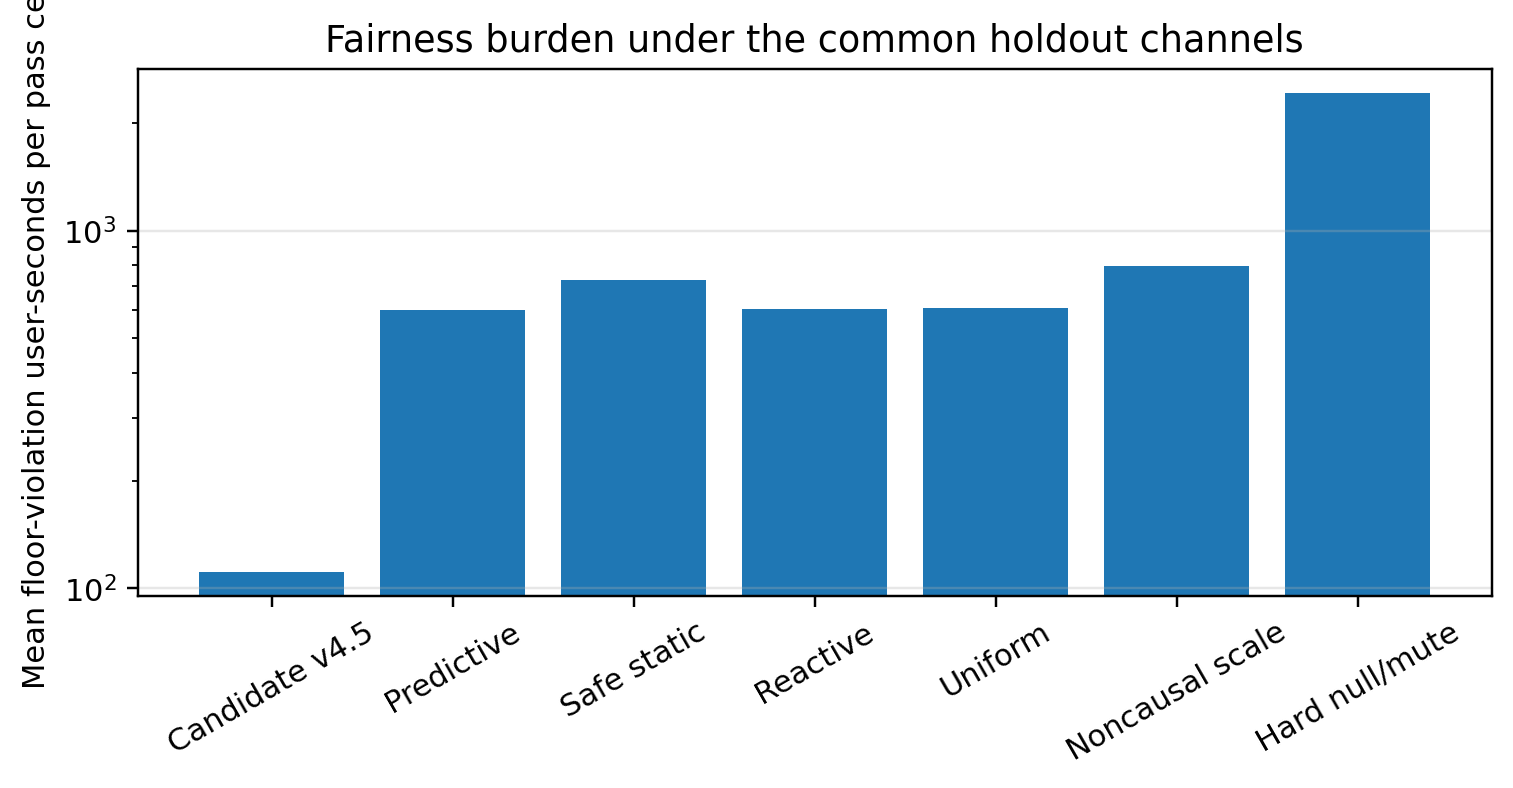
\includegraphics[width=\columnwidth]{figures/holdout_floor_burden.png}
\caption{Mean floor-violation user-seconds per pass cell. The log scale exposes the large penalty of hard null/mute and the reduction obtained by the candidate hierarchy.}
\label{fig:floor-burden}
\end{figure}

\subsection{Fairness and fixed-association serviceability}
The candidate has zero floor violations in 17 of 30 fresh seeds. Across all 30 seeds it records 16,646 floor-violation user-seconds and 3,340 floor-violation user-intervals, reducing the burden by 81.47\% relative to predictive control and 84.76\% relative to safe static. The maximum normalized shortfall is 57.26\%, and 1,328 intervals remain unresolved within the declared scheduling library.

The residual is a major limitation but not an incumbent-safety failure. Prior exact diagnosis found no fixed-beam single-user infeasible interval: every affected user can be served when sufficiently protected. Most difficult intervals instead exhibit joint simultaneous-transmission incompatibility under fixed association and bounded coordination. Target-only scheduling closed roughly 70\% of the earlier unresolved intervals, whereas the companion-aware extension closed only four additional development intervals. That negligible marginal gain motivated the pre-specified stopping decision and the fresh holdout rather than an endless sequence of post-hoc mode libraries.

The correct interpretation is therefore feasibility conditioned. When the hierarchy returns a witness, the unchanged floor and EESS constraints are audited. When it does not, the controller reports the shortfall and the paper identifies association/admission as the missing degree of freedom.


\subsection{Development evolution and stopping rule}
\begin{table}[t]
\caption{Development-only evolution of the floor-feasibility hierarchy. The fresh holdout uses frozen v4.5.}
\label{tab:development-ablation}
\centering
\footnotesize
\setlength{\tabcolsep}{3.0pt}
\renewcommand{\arraystretch}{1.06}
\begin{tabular}{@{}lrr@{}}
\toprule
Candidate & Unresolved intervals & Floor user-sec.\\
\midrule
v4.3: fixed-beam repair & $1{,}736$ & $19{,}994$\\
v4.4: target scheduling & $523$ & $6{,}540$\\
v4.5: companion-aware scheduling & $519$ & $6{,}505$\\
\bottomrule
\end{tabular}
\end{table}

The original reviewed predictive controller had zero EESS violations on the excluded development smoke but 519 floor-violation user-seconds. Candidate v4.3 closed that smoke by adding exact fixed-beam power repair. In the 30-seed development campaign, v4.3 retained 1,736 unresolved intervals. Exact diagnosis classified 1,284 of them as jointly infeasible for simultaneous fixed-beam power allocation, while no affected user was individually infeasible.

Candidate v4.4 introduced target-focused protected-subband scheduling and reduced the development residual to 523 intervals. Candidate v4.5 completed the companion singleton basis but closed only four more intervals, leaving 519. The marginal closure of 0.76\% was pre-specified as the point to stop mode-library tuning. The fresh holdout therefore tests a frozen v4.5 rather than an algorithm repeatedly adapted to every difficult seed.

This evolution provides an ablation narrative: prediction supplies EESS safety, stream-power repair corrects same-sector imbalance, scheduling convexifies joint service, and residual fixed-association serviceability defines the limitation. It also explains why the paper does not proceed to a v4.6 scheduling library.

\subsection{Pass robustness}
\begin{figure}[t]
\centering
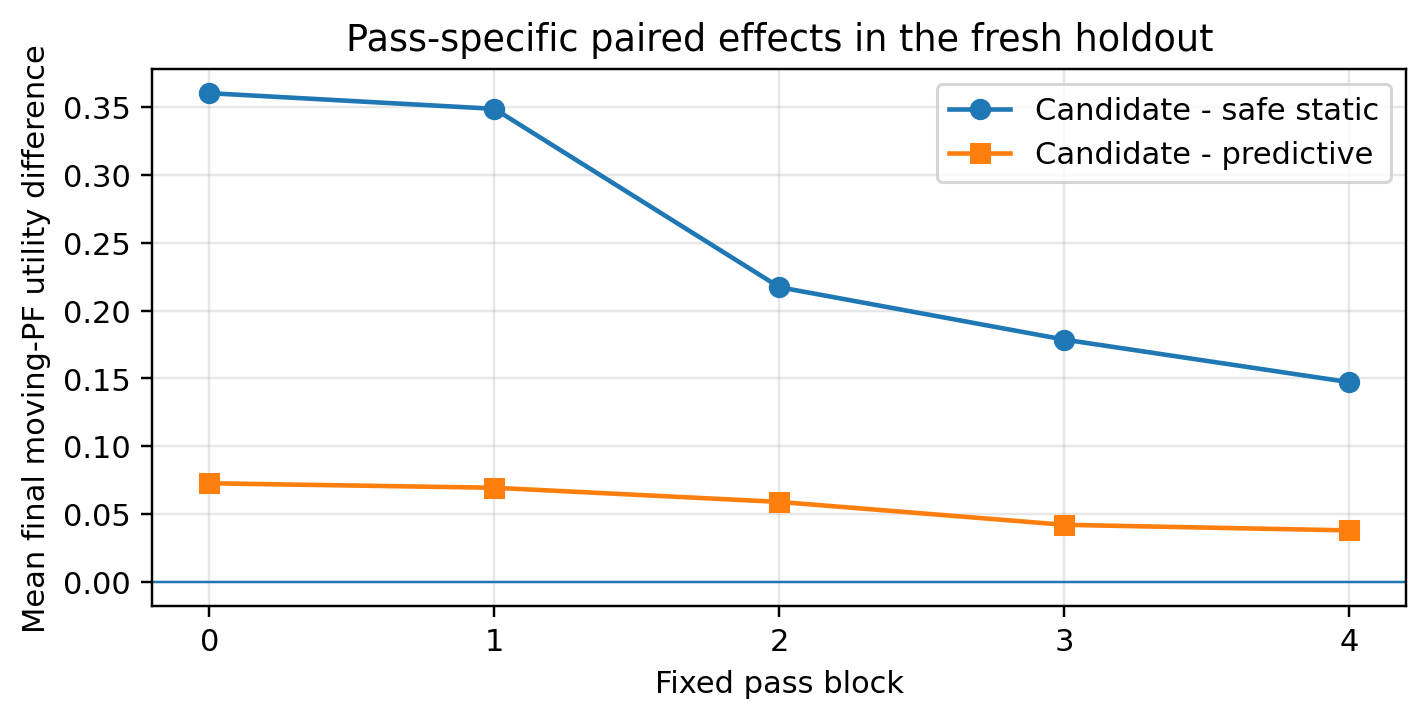
\includegraphics[width=\columnwidth]{figures/holdout_pass_effects.png}
\caption{Mean pass-specific final moving-PF effects in the fresh holdout.}
\label{fig:pass-effects}
\end{figure}

The candidate-minus-static final-PF mean is positive in each fixed pass block. Leave-one-pass-out seed-cluster intervals also remain strictly positive: the five lower endpoints range from 0.1753 to 0.2212. The candidate-minus-predictive pass means are positive, although individual seed-pass effects can be negative; the seed-cluster aggregate remains positive. This is consistent with a controller that improves average moving fairness without claiming pointwise dominance.


The width of the seed-cluster interval reflects meaningful topology-to-topology variation. For candidate minus safe static, the seed-level final-PF effect has standard deviation 0.156, with observed effects from 0.043 to 0.836. For candidate minus predictive, the seed-level range includes negative values even though the mean and confidence interval are positive. The proper inference is therefore population-average superiority under the frozen seed design, not universal seedwise improvement.

The mandatory duration-weighted endpoint reaches the same conclusion. Its candidate-minus-static interval is $[0.1767,0.2415]$, and its candidate-minus-predictive interval is $[0.0078,0.0652]$. Agreement between final and duration-weighted endpoints reduces the risk that the result is driven only by the terminal moving-rate state.

\section{Complexity, Locality, and Practicality}
\begin{table}[t]
\caption{Reference-computation distribution and fallback incidence.}
\label{tab:runtime-v2}
\centering
\footnotesize
\setlength{\tabcolsep}{3.0pt}
\renewcommand{\arraystretch}{1.05}
\begin{tabular}{@{}lr@{}}
\toprule
Metric & Value\\
\midrule
End-to-end per pass, median & $2.09$ s\\
End-to-end per pass, 95th percentile & $49.01$ s\\
End-to-end per pass, maximum & $794.8$ s\\
Fixed-beam LP maximum & $0.226$ s\\
Scheduling attempts / all intervals & $1,834/17,700$ ($10.4\%$)\\
Feasible schedules / attempts & $506/1,834$ ($27.6\%$)\\
Maximum scheduling modes & $7,776$\\
Maximum mutable sectors & $9$\\
\bottomrule
\end{tabular}
\end{table}


\begin{figure}[t]
\centering
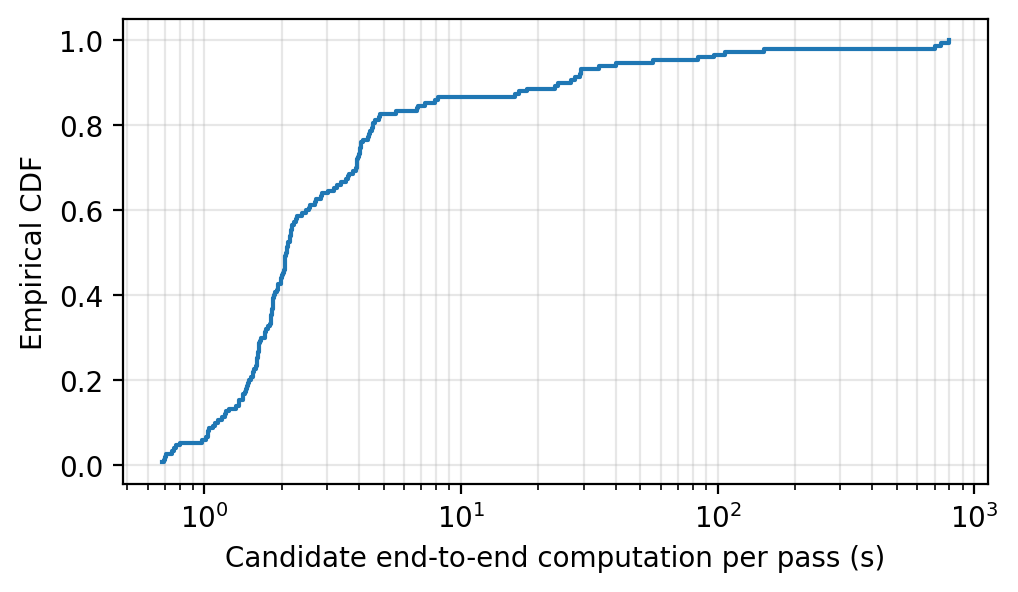
\includegraphics[width=\columnwidth]{figures/holdout_runtime_ecdf.png}
\caption{Empirical distribution of candidate end-to-end reference computation per seed--pass cell. The logarithmic abscissa separates the common fixed-beam path from rare large scheduling libraries.}
\label{fig:runtime-ecdf}
\end{figure}

The median reference computation is 2.09 s per pass cell and the 95th percentile is 49.01 s. The normal fixed-beam LP has a 0.226-s maximum. Protected-subband scheduling is attempted in 1,834 of 17,700 candidate intervals (10.4\%); 506 of those attempts return feasible schedules. Thus the expensive combinatorial layer is exceptional rather than the normal operating path. The maximum 794.8-s pass and 7,776-mode library arise from one difficult fixed-association case and motivate the archived pass-parallel recovery.

These measurements come from an unoptimized Python/SciPy/HiGHS reference implementation. They support an offline feasibility benchmark and a practical fast path, not a claim that the complete enumerative fallback is already a near-real-time xApp. A deployable realization would retain the same action semantics but use mode pruning, column generation, warm starts, cached templates, or a slower supervisory timescale.

The action itself is bounded and structured: the candidate uses at most eight guard sectors and nine mutable sectors, retains fixed RZF directions, satisfies strict post-mode power, and never needs deployable $q=0$ headroom. The archived lower bound on incremental control payload is 191,540 bytes over 150 candidate pass cells, with 18,593 changed sector-intervals and 45,149 changed stream coefficients. This is an action-count lower bound, not a serialized protocol measurement. Action-scope locality is verified; standardized message timing and reliability are not.

\subsection{Control-plane contract}
The simulator separates action locality from information-exchange certification. A normal sector reports a small local action table and predicted leakage contribution; the coordinator returns two protected-mode attenuations and, when needed, a sparse sector scale. Fixed-beam repair adds stream coefficients only for the explicit mutable set. Scheduling returns a finite mode mixture and guard list for the protected group. In the fresh holdout, the union of mutable sectors never exceeds nine and scheduling is attempted in only 10.4\% of intervals.

The archived payload lower bound counts four bytes per changed stream coefficient, four bytes per nonzero scheduling-mode entry, and two bytes per mutable schedule sector. It omits headers, identifiers, reliability procedures, quantization design, and transport protocol. Consequently, the evidence supports bounded action cardinality and an implementation target, but not a standardized latency or fronthaul-throughput claim.

\subsection{Deployment interpretation}
The measured distribution suggests a two-timescale implementation. Predictive sector selection and the fixed-beam LP form the normal 5-s control path. A large scheduling library is a rare supervisory fallback and can be precomputed, decomposed, or invoked on a slower timescale when repeated serviceability failures are detected. This interpretation preserves the evaluated radio actions while avoiding the unsupported claim that full mode enumeration must finish inside every 5-s interval.

The controller requires no future user small-scale channel beyond the simulated current realization; prediction concerns the protected-pass coupling and command reachability. A deployment would therefore combine a slowly refreshed incumbent database/pass forecast with local channel estimation and PF state. Database error, transport delay beyond the declared one-update model, and hardware null-depth uncertainty remain engineering validation items rather than hidden assumptions.

The utility effects should also be interpreted in system context. Only the central 10 MHz of a 100-MHz allocation is directly controlled by the protected-subband hierarchy. A network-wide final moving-PF difference of 0.2505 over safe static is consequently moderate in absolute scale but statistically stable and accompanied by an 84.76\% reduction in floor burden. The result is operationally meaningful without being portrayed as an order-of-magnitude capacity gain.

\section{Discussion}
\subsection{Why the utility gain survives the holdout}
The candidate's primary gain over safe static is not produced by violating incumbent limits: both methods have zero EESS violations. It is also not produced by a larger power envelope: the candidate passes the strict post-mode power gate and uses no deployable $q=0$ headroom. The gain comes from temporal prediction and selective actions that avoid the persistent conservatism of a static setting.

The smaller but positive gain over the reviewed predictive controller has a different origin. Both methods use future coupling and the same safety logic, but the candidate can redistribute fixed-beam stream power and schedule protected-subband service when a sector-common action is inadequate. The candidate-minus-predictive final-PF confidence interval remains positive even though some individual seed effects are negative. Thus, the evidence supports average improvement under the seed population, not deterministic dominance.

\subsection{Interpretation of residual floors}
A universal floor theorem would require an explicit serviceability assumption, a broader action class, or an admission/association mechanism. None is imposed here. The residual 13 seeds show that no accepted witness exists in the declared finite, fixed-association bounded-local action class for every interval. This is not a proof that the floor is physically impossible under arbitrary reassociation or beam redesign. Because every diagnosed affected user was individually serviceable, the natural next extension is association or multi-connectivity rather than a weaker floor.

For the present paper, feasibility conditioning is preferable to post-hoc admission. It leaves the fairness policy unchanged, quantifies the residual, and makes the action boundary reproducible. The candidate can still be attractive operationally because it cuts floor burden by more than 80\% while preserving utility and EESS safety.

\subsection{What is and is not ``distributed''}
The beamforming and normal action evaluation are local; the coordinator handles an incumbent price and a sparse list of critical sectors. Accepted actions modify a bounded sector set. This is sufficient to call the action architecture bounded-local. However, the simulator has not measured the complete message schedule, transport delay, or failure behavior of a standardized deployment. We therefore avoid claiming an implemented O-RAN xApp or certified distributed protocol.

\section{Limitations and Claim Boundaries}
The study has four principal boundaries.
\begin{enumerate}
\item The 65-dB null-depth cap and 3-dB coupling uplift are declared engineering envelopes, not hardware-calibrated confidence bounds.
\item P.452/SA.1027/SA.509 are used in a documented engineering scenario. The results are not a licensing or regulatory-compliance certificate.
\item The controller's user-floor guarantee is conditional on feasibility within the fixed-association bounded action class. Thirteen of 30 fresh seeds retain at least one floor violation.
\item The scheduling reference implementation is not yet certified for near-real-time deployment, and information-exchange locality is not fully measured.
\end{enumerate}
These boundaries do not invalidate the primary contribution. The fresh holdout demonstrates statistically significant utility improvement and complete EESS safety under the declared model, while the unresolved floor cases identify a precise architectural frontier. User reassignment, multi-connectivity, and serviceability-aware admission are the appropriate next scientific extensions rather than further small modifications to the same mode library.

\section{Reproducibility}
Each seed return binds the topology/channel seed, exact candidate source manifest, five pass records, all nine methods, environment, and per-file hashes. One channel is generated per seed and reused across passes and methods. The final fresh-holdout archive contains 30 seed results, 1,350 method-pass cells, seed-cluster effects, pass-specific effects, leave-one-pass-out analysis, 10,000-replication bootstrap summaries, Slurm evidence, and a portable SHA-256 manifest. Candidate v4.5 was frozen before seeds 44030--44059 were evaluated, and no automatic extra seeds or algorithm tuning were authorized afterward.

\section{Conclusion}
A predictive constrained-PF controller with bounded local actions can protect a simulated EESS incumbent under delayed and slew-limited FR3 operation while improving moving fairness utility over safe static and reviewed predictive baselines. Exact fixed-beam power repair and protected-subband scheduling greatly reduce user-floor failures without changing beam directions, weakening the floor, or violating strict post-mode power. A fresh 30-seed holdout yields a candidate-minus-static final-PF effect of $0.2505$ with 95\% interval $[0.2013,0.3102]$ and zero long- or short-horizon EESS violations in all 150 candidate pass cells. The unchanged floor is not universally feasible under fixed association, so the paper makes a feasibility-conditioned service claim and reports certified shortfall. This combination of strong positive results and explicit limits provides a defensible basis for FR3 coexistence control and exposes association-aware serviceability as the next major research problem.


\appendices
\section{Derivation of the Fixed-Beam Floor Rows}
Let the total rate be $R_{u}=R^{\rm other}_{u}+\omega_p\log_2(1+\mathrm{SINR}_{u})$, where $\omega_p$ is the protected-subband weight. If $F_u\le R^{\rm other}_u$, no protected-rate row is needed. Otherwise,
\begin{equation}
 \gamma_u=2^{(F_u-R^{\rm other}_u)/\omega_p}-1.
\end{equation}
With desired gain $g_{u,d}$ and stream scales $x_j$,
\begin{align}
 \frac{g_{u,d}x_d}{\sum_{j\ne d}g_{u,j}x_j+N_0}&\ge\gamma_u\\
 \gamma_u\sum_j g_{u,j}x_j-(\gamma_u+1)g_{u,d}x_d
 &\le-\gamma_u N_0.
\end{align}
The implementation positively rescales each row for numerical conditioning but does not alter the inequality or introduce a floor tolerance. EESS rows are constructed for every physical second by multiplying the sector-stream leakage by the criterion-specific coupling and dividing by the allowance.

\section{Schedule Construction and Audit}
For each unresolved interval, critical sectors are those serving pre-scheduling violating users. Candidate v4.4 generated baseline and target singleton options. Candidate v4.5 additionally generates singleton options for active companion streams in the critical sectors. A global guard set is ranked from external interference and EESS contribution. All nonbaseline modes use a bounded subset, so the union of mutable guards cannot silently grow across modes.

Every mode is audited for coefficients in $[0,1]$, post-mode sector power, user rates, and long/short EESS ratios. The continuous LP first establishes fractional feasibility with interior reserves. The integer master converts fractions to exactly 2,000 half-millisecond slots. The accepted integer schedule is re-evaluated from its slot fractions; success requires zero floor and EESS violations under the unchanged scientific comparison tolerances.

\section{Seed-Cluster Bootstrap}
Let $D_i$ be the average of the five fixed pass effects for seed $i$. For each endpoint, the point estimate is $\bar D=30^{-1}\sum_iD_i$. The bootstrap samples 30 seed indices with replacement, averages their $D_i$, and repeats this procedure 10,000 times. The reported interval is the 2.5th and 97.5th percentiles. Passes are not resampled because they are fixed geometry/load blocks. The leave-one-pass-out analysis removes one block from every seed before repeating the seed-cluster bootstrap.


\section{Reference Complexity Decomposition}
At fixed beams, the LP has one variable per active sector-stream multiplier in the mutable scope, one floor row per active eligible user requiring protected-band support, two sets of physical-second EESS rows, and sector power rows. Its size is therefore modest in the evaluated local scope.

The scheduling fallback is combinatorial in the number of per-sector options. If critical sector $b$ has $q_b$ options, the unpruned Cartesian library contains $\prod_b q_b$ modes before duplicate removal. Seed 44052 reaches 7,776 modes and motivates the archived implementation-capacity and pass-parallel recovery. This is a reference-computation issue rather than a new scientific action. A deployable implementation should exploit column generation, guard-set decomposition, or cached templates rather than enumerate the full library online.

\section{Finite-Pass Reachability Induction}
For one criterion, write $\bm z_i=10^{-\bm q_i/10}$ and let $\langle\cdot,\cdot\rangle$ denote the sector--mode inner product. The envelope recurrence gives $\bm h_i\succeq\overline{\bm c}_i$ and $\bm h_i\succeq\alpha\bm h_{i+1}$. If the command applied in interval $i$ was selected $d$ updates earlier and obeys the slew constraint, then its attenuation vector dominates the reachable attenuation assumed by the shifted envelope. Hence
\begin{equation}
 \langle\overline{\bm c}_i,\bm z_i\rangle
 \le \langle\bm h_i,\bm z_i\rangle
 \le A_i.
\end{equation}
The base case is the preloaded action screened against $\bm h_0$. Applying the recurrence proves the result for each subsequent interval. The implementation independently checks the recurrence excess, command slew, selected-envelope ratio, realized upper-envelope ratio, terminal maximum-action feasibility, and fail-safe recursive candidate.

\section{Frozen Holdout and Reproducibility Contract}
The development seeds are 44000--44029; the fresh holdout seeds are 44030--44059. For campaign seed $s$, the cellular-user seed is $2s$ and the channel seed is $2s+1$. One full topology/channel bundle is generated per seed and reused by all five fixed pass blocks and all nine methods. This common-random-number construction makes every utility and floor comparison paired within seed.

Candidate v4.5, the method list, primary and mandatory secondary endpoints, seed list, pass definitions, bootstrap procedure, hard safety gates, and feasibility-conditioned claim were committed before holdout execution. Scientific nonzero exits and infrastructure recoveries remain in the archive; no seed is replaced based on outcome. Each return binds the channel record, source manifest, environment, result-file hashes, and Slurm record. These measures support computational reproduction of the reported engineering scenario but do not turn the scenario into a regulatory certificate.

\section{Claim Checklist}
The evidence supports: (i) zero long- and short-horizon EESS violations in all fresh candidate cells under the declared model; (ii) positive paired utility effects over safe static and reviewed predictive controls; (iii) strict post-mode power and bounded action-scope compliance; and (iv) large floor-burden reductions.

The evidence does not support: hardware-calibrated null depth, regulatory compliance, a universal floor guarantee, measured standardized signalling overhead, or a near-real-time implementation of the full scheduling enumeration. These exclusions are part of the scientific result, not optional wording.

\begin{thebibliography}{99}
\bibitem{zhao2007dsa} Q. Zhao and B. M. Sadler, ``A survey of dynamic spectrum access,'' \emph{IEEE Signal Process. Mag.}, vol. 24, no. 3, pp. 79--89, May 2007.
\bibitem{ghasemi2007limits} A. Ghasemi and E. S. Sousa, ``Fundamental limits of spectrum-sharing in fading environments,'' \emph{IEEE Trans. Wireless Commun.}, vol. 6, no. 2, pp. 649--658, Feb. 2007.
\bibitem{zhang2008multiantenna} R. Zhang and Y.-C. Liang, ``Exploiting multi-antennas for opportunistic spectrum sharing in cognitive radio networks,'' \emph{IEEE J. Sel. Topics Signal Process.}, vol. 2, no. 1, pp. 88--102, Feb. 2008.
\bibitem{christensen2008weighted} S. S. Christensen, R. Agarwal, E. de Carvalho, and J. M. Cioffi, ``Weighted sum-rate maximization using weighted MMSE for MIMO-BC beamforming design,'' \emph{IEEE Trans. Wireless Commun.}, vol. 7, no. 12, pp. 4792--4799, Dec. 2008.
\bibitem{shi2011wmmse} Q. Shi, M. Razaviyayn, Z.-Q. Luo, and C. He, ``An iteratively weighted MMSE approach to distributed sum-utility maximization for a MIMO interfering broadcast channel,'' \emph{IEEE Trans. Signal Process.}, vol. 59, no. 9, pp. 4331--4340, Sept. 2011.
\bibitem{wagner2012large} S. Wagner, R. Couillet, M. Debbah, and D. T. M. Slock, ``Large system analysis of linear precoding in correlated MISO broadcast channels under limited feedback,'' \emph{IEEE Trans. Inf. Theory}, vol. 58, no. 7, pp. 4509--4537, July 2012.
\bibitem{rawlings2017mpc} J. B. Rawlings, D. Q. Mayne, and M. M. Diehl, \emph{Model Predictive Control: Theory, Computation, and Design}, 2nd ed. Madison, WI, USA: Nob Hill, 2017.
\bibitem{ames2017cbf} A. D. Ames, X. Xu, J. W. Grizzle, and P. Tabuada, ``Control barrier function based quadratic programs for safety critical systems,'' \emph{IEEE Trans. Autom. Control}, vol. 62, no. 8, pp. 3861--3876, Aug. 2017.
\bibitem{ames2019theory} A. D. Ames, S. Coogan, M. Egerstedt, G. Notomista, K. Sreenath, and P. Tabuada, ``Control barrier functions: Theory and applications,'' in \emph{Proc. Eur. Control Conf.}, 2019, pp. 3420--3431.
\bibitem{agrawal2017dcbf} A. Agrawal and K. Sreenath, ``Discrete control barrier functions for safety-critical control of discrete systems,'' in \emph{Proc. Robotics: Science and Systems}, 2017.
\bibitem{jankovic2018robust} M. Jankovic, ``Robust control barrier functions for constrained stabilization of nonlinear systems,'' \emph{Automatica}, vol. 96, pp. 359--367, 2018.
\bibitem{xiao2022hocbf} W. Xiao and C. Belta, ``High-order control barrier functions,'' \emph{IEEE Trans. Autom. Control}, vol. 67, no. 7, pp. 3655--3662, July 2022.
\bibitem{boyd2004convex} S. Boyd and L. Vandenberghe, \emph{Convex Optimization}. Cambridge, U.K.: Cambridge Univ. Press, 2004.
\bibitem{hoydis2022sionna} J. Hoydis \emph{et al.}, ``Sionna: An open-source library for next-generation physical layer research,'' arXiv:2203.11854, 2022.
\bibitem{kang2024upper} S. Kang \emph{et al.}, ``Cellular wireless networks in the upper mid-band,'' \emph{IEEE Open J. Commun. Soc.}, 2024.
\bibitem{chamberlain2024sharing} J. Chamberlain, D. Starobinski, and J. T. Johnson, ``Facilitating spectrum sharing with passive satellite incumbents,'' \emph{IEEE J. Sel. Areas Commun.}, 2024.
\bibitem{3gpp38901} 3GPP, ``Study on channel model for frequencies from 0.5 to 100 GHz,'' TR 38.901, V19.4.0, 2026.
\bibitem{iturp452} ITU-R, ``Prediction procedure for the evaluation of interference between stations on the surface of the Earth at frequencies above about 0.1 GHz,'' Rec. P.452-18, 2023.
\bibitem{itursa1027} ITU-R, ``Sharing criteria for space-to-Earth data transmission systems in the Earth exploration-satellite and meteorological-satellite services using satellites in low-Earth orbit,'' Rec. SA.1027-6, 2019.
\bibitem{itursa509} ITU-R, ``Space research earth station and radio astronomy reference antenna radiation pattern for use in interference calculations,'' Rec. SA.509, 2013.
\bibitem{iturf758} ITU-R, ``System parameters and considerations in the development of criteria for sharing or compatibility involving the fixed service,'' Rec. F.758-8, 2025.
\bibitem{ised3077} Innovation, Science and Economic Development Canada, ``Technical requirements for fixed line-of-sight radio systems operating in the band 7725--8275 MHz,'' SRSP-307.7, Issue 6, 2006.
\bibitem{itursa1023} ITU-R, ``Methodology for determining sharing and coordination criteria for systems in the Earth exploration-satellite and meteorological-satellite services,'' Rec. SA.1023-1, 1999.
\bibitem{iturp452validation} ITU-R Study Group 3, ``Validation examples for software implementation of Recommendation ITU-R P.452-18,'' Version 18.0, 2023.
\bibitem{sionna201docs} NVIDIA, ``Sionna 2.0.1 documentation: 3GPP TR 38.901 Urban Macrocell channel model,'' 2026.
\end{thebibliography}

\end{document}
